\section{Optimization}
\label{sec:optimization}

Due to the high cost of proxy re-encryption operations, which we discussed in \S\ref{sec:evaluation}, we investigated Go's compiler optimizations on the \texttt{pre} library, with the hopes of understanding its runtime.
This is discussed in \S\ref{sec:compiler-optimizations}.
The performance results are discussed in \S\ref{sec:optimization-results}.

\subsection{Compiler Optimizations}
\label{sec:compiler-optimizations}

The Go compiler is intentionally opinionated and ships with a set of aggressive default optimizations that cannot be tuned by developers via traditional \texttt{-O} flags like in C/C++.
These default optimizations include inlining of small functions, escape analysis to avoid heap allocations, dead code elimination, constant folding, and SSA (static single assignment) form for better register allocation.
As such, most Go binaries are highly optimized out of the box, and further improvements require either rewriting code or disabling these defaults for comparison purposes, which is what we do.

To understand the contribution of these compiler optimizations to the performance of the \texttt{pre} library, we benchmark four different compiler configurations:

\begin{itemize}
  \item \textbf{Default:} Standard Go compiler output with all optimizations enabled.
  \item \textbf{Noinline:} (\texttt{-gcflags=all=-l}) Compiled with function inlining disabled.
  \item \textbf{Noopt:} (\texttt{-gcflags=all=-N -l}) Compiled with all optimizations disabled.
  \item \textbf{Race:} (\texttt{-race}) Compiled with the Go race detector enabled, which instruments memory accesses for concurrency analysis.
\end{itemize}


\subsection{Results}
\label{sec:optimization-results}

\begin{figure}
    \centering
    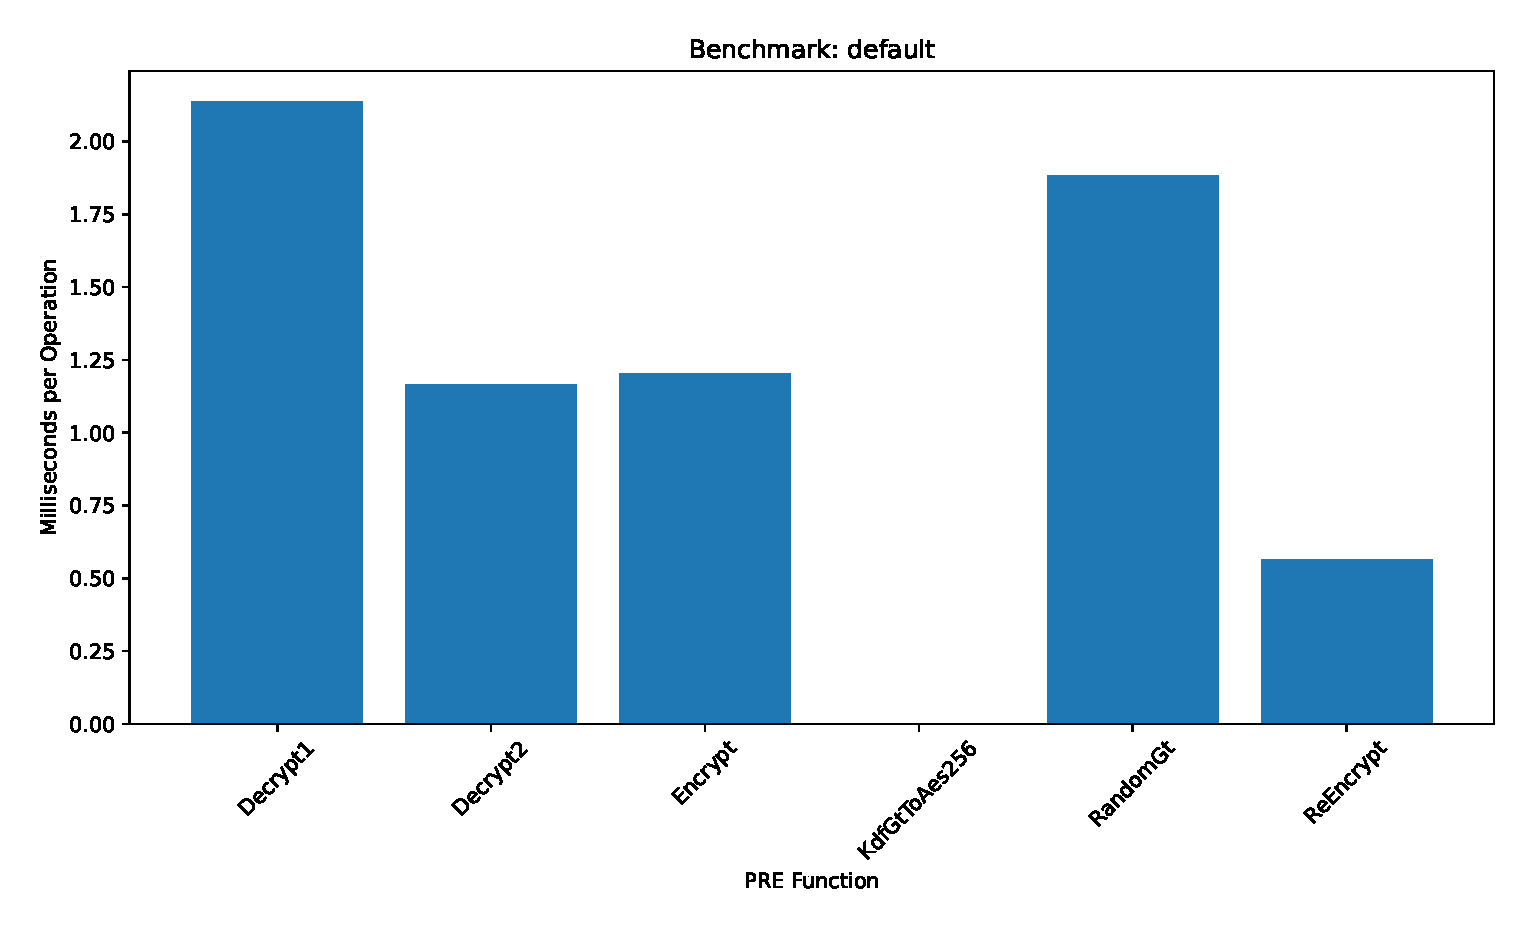
\includegraphics[width=0.48\textwidth]{figs/bench_default}
    \caption{Benchmark results for the \texttt{pre} library under default Go compiler settings.}
    \label{fig:bench-default}
\end{figure}

\begin{figure}
    \centering
    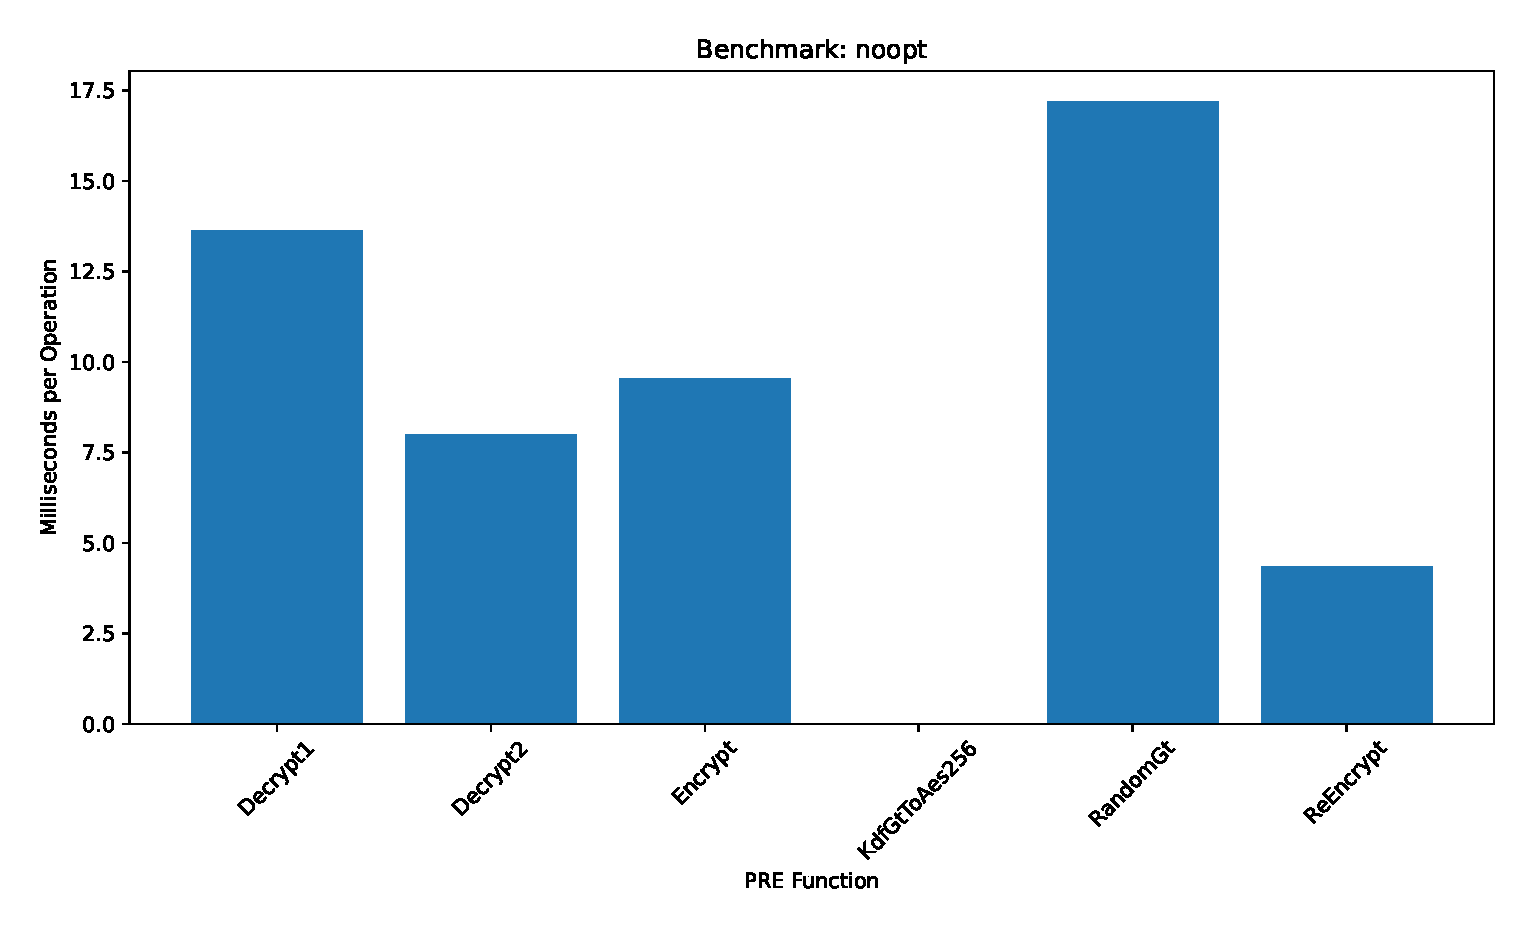
\includegraphics[width=0.48\textwidth]{figs/bench_noopt}
    \caption{Benchmark results for the \texttt{pre} library with optimizations disabled (-gcflags=all=-N -l).}
    \label{fig:bench-noopt}
\end{figure}

\begin{figure}
    \centering
    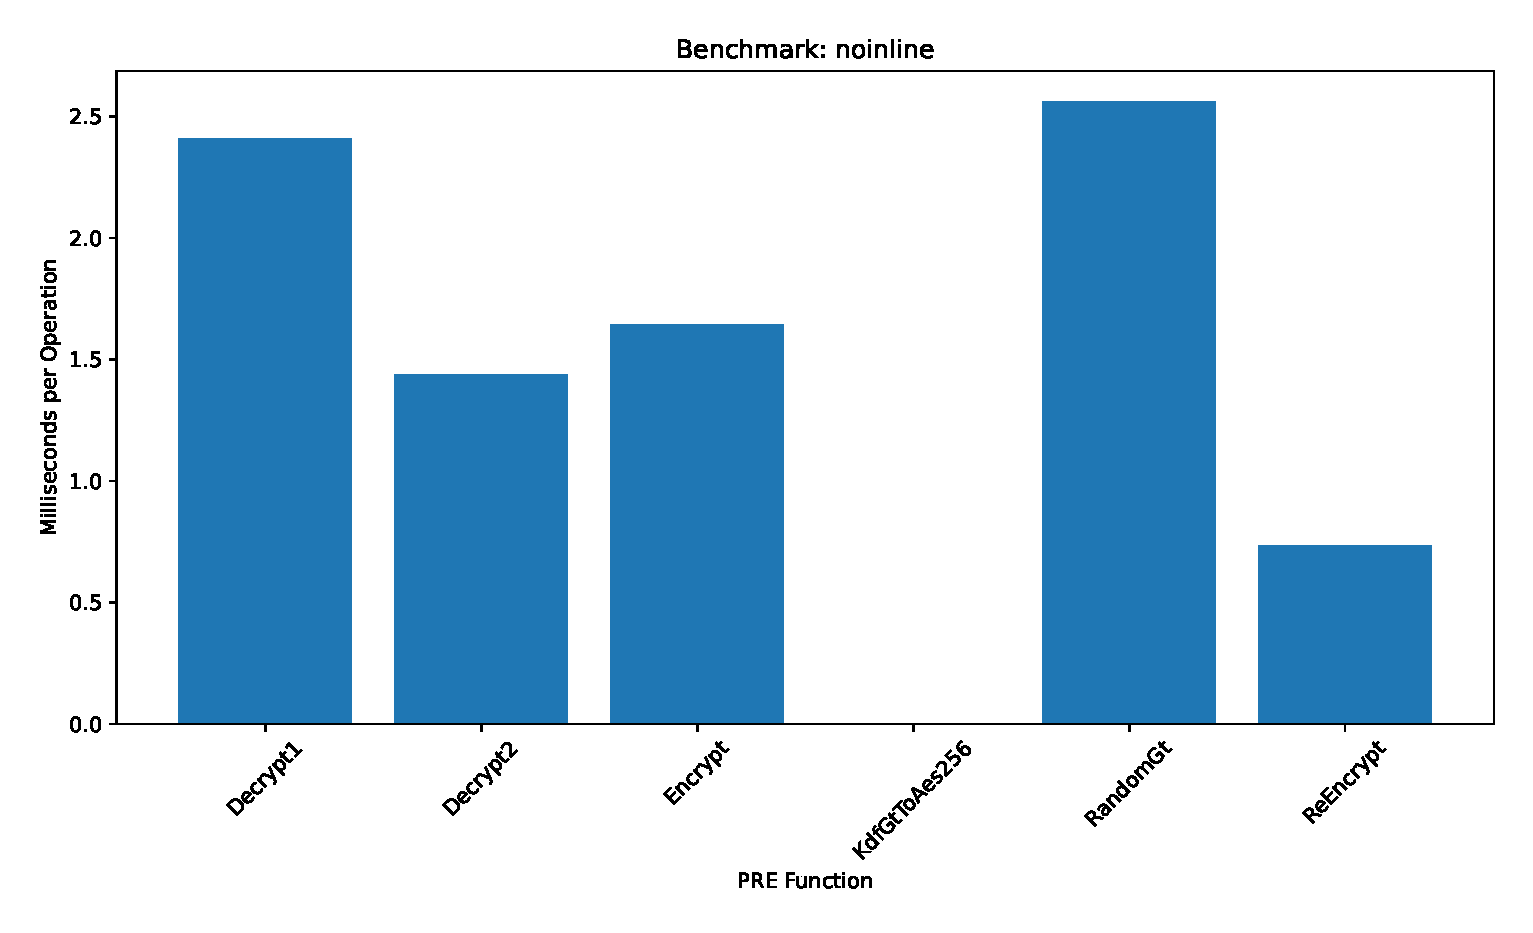
\includegraphics[width=0.48\textwidth]{figs/bench_noinline}
    \caption{Benchmark results for the \texttt{pre} library with inlining disabled (-gcflags=all=-l).}
    \label{fig:bench-noinline}
\end{figure}

\begin{figure}
    \centering
    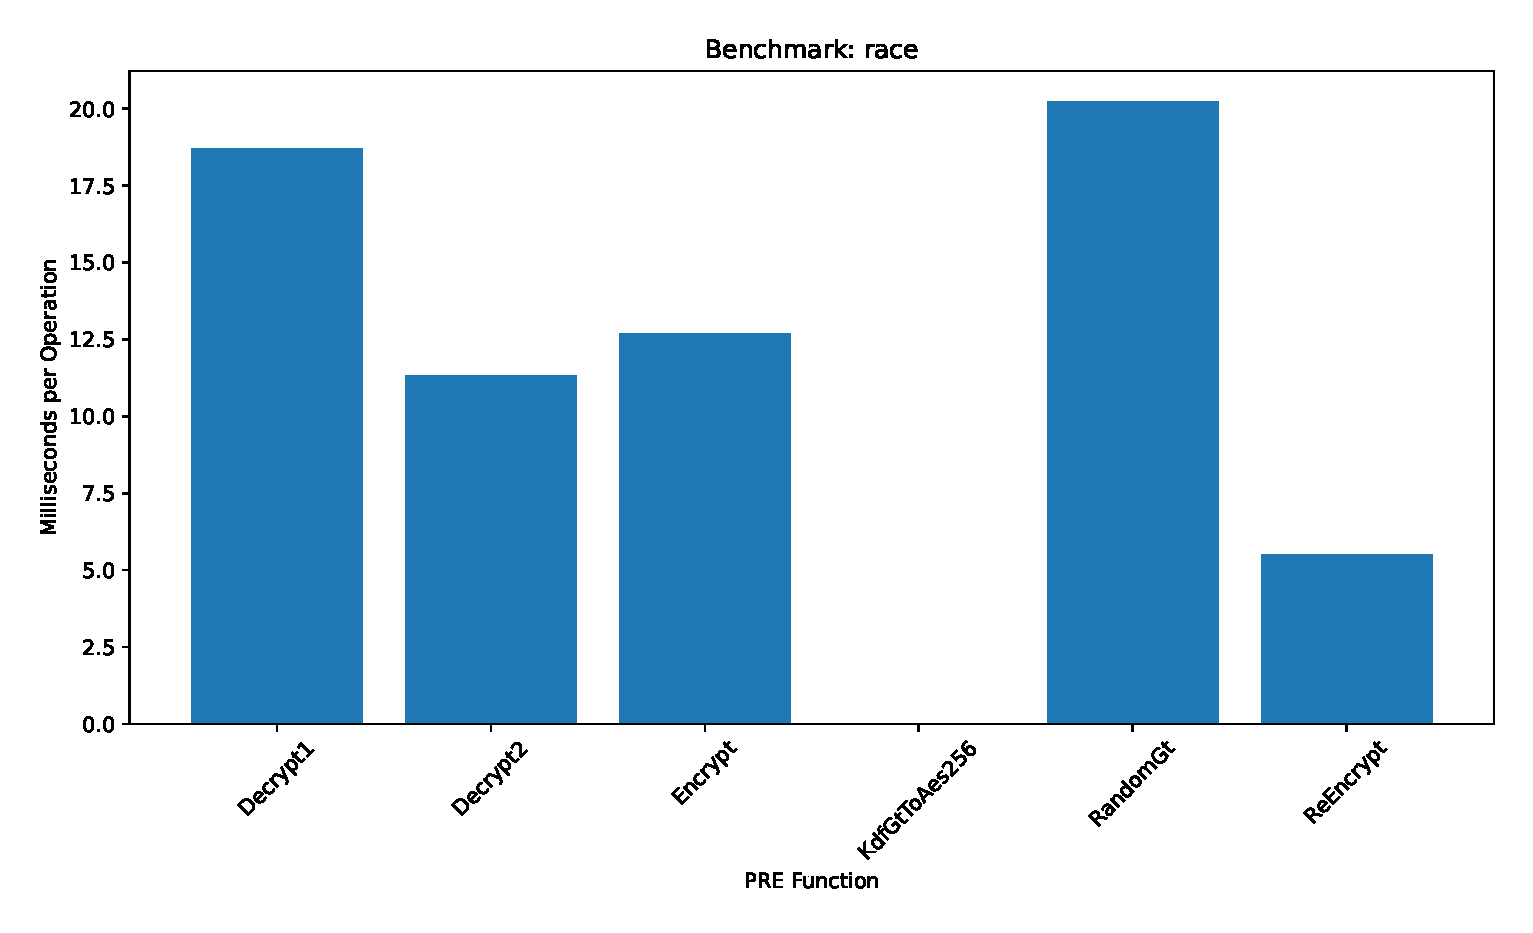
\includegraphics[width=0.48\textwidth]{figs/bench_race}
    \caption{Benchmark results for the \texttt{pre} library compiled with the race detector enabled.}
    \label{fig:bench-race}
\end{figure}

As expected, the Go compiler’s default output significantly outperforms the less-optimized builds.
We re-run the benchmarks with default settings for the purpose of directly comparing against other optimization states, and show the results in Figure~\ref{fig:bench-default}

Disabling all optimizations (\texttt{noopt}) results in an average slowdown of more than $7\times$ across all measured functions.
These results can be seen in Figure~\ref{fig:bench-noopt}.
The most affected function is \texttt{pre.RandomGt}, which takes $1.88$ ms in the default build and balloons to $17.18$ ms with optimizations disabled. 
This is a slowdown of over $9\times$.
Similarly, \texttt{Encrypt} and \texttt{ReEncrypt} become $7.9\times$ and $7.7\times$ slower respectively in the \texttt{noopt} build.

Disabling only inlining (\texttt{noinline}) has a smaller, but still measurable, effect, as seen in Figure~\ref{fig:bench-noinline}.
All functions slow down by roughly $30-35\%$, confirming that inlining is one of the most impactful individual optimizations in this context, affecting all functions more evenly than some other optimizations we compare.
Even \texttt{Decrypt1}, which is relatively simple, ran about $12.8\%$ slower without inlining.

Finally, enabling the Go race detector (\texttt{race}) produced a $9\times$ slowdown on average, which we see in Figure~\ref{fig:bench-race}
This is unsurprising, as the race detector instruments every read and write with additional bookkeeping to detect concurrent access violations.

These results reaffirm that the Go compiler’s default configuration is already highly optimized for performance.
They also validate our use of Go for cryptographic code, as the compiler produces competitive results without requiring manual tuning.

